\chapter{Background}

\section{CSR Storage Format}
CSR (Compressed Sparse Row) is the most widely used storage format for sparse matrices. As its name suggests, it compresses the amount of memory used to store a matrix without loss of information. It does so by utilizing three vectors \(A_{p}, A_{j}, A_{x}\). Figure \ref{fig:csrformat} shows an example of a matrix stored in CSR format, adapted from \cite{gupta2024gamgi}.

\begin{figure}[ht]
    \centering
    \incfig{csrformat}
    \caption{Matrix represented in the CSR format.}
    \label{fig:csrformat}
\end{figure}

The first vector, \(A_{p}\) stores the indices of the first non-zero in the vectors \(A_{p}\) and \(A_{x}\). For a given entry \(A_{p}[i]\), \(A_{p}[i]\) is the index of the first non-zero in the \(i^{\text{th}}\) row. \(A_{j}[j]\) and \(A_{x}[j]\) denotes the column index and value of the \(j^{\text{th}}\) non-zero, respectively.
\medskip

Throughout the remainder of this thesis, we operate under the assumption that all matrices are represented in CSR format, unless explicitly noted otherwise.


\subsection{Computational Intensity}

The \textit{computational intensity} of an operation describes the relation between the number of floating-point operations (FLOPS) and the number of memory accesses required. It is formally defined as:

\begin{equation}
    \text{Computational intensity} = \frac{\text{FLOPS}}{\text{Memory accesses}}
    \label{eq:computationaldensity}
\end{equation}

Operations with low computational intensity, such as SpMV, are often \textit{memory bound} rather than \textit{compute bound}. This means that increasing the computational power of a system (e.g., faster processors) does not necessarily lead to proportional speedups in SpMV performance, as memory bandwidth remains the limiting factor.

\section{Other storage formats}
There are of course other ways to store a matrix, each with their own benefits and drawbacks.

\subsection{COO Format}
The Coordinate List (COO) format stores the matrix as a set of triples on the form \(i,j,x\), where \(i\) is the row index, \(j\) is the column index, and \(x\) is the value stored at \((i,j)\) in the matrix. In this format all \(0\) entries are ignored.

\begin{figure}[H]
    \centering
    \incfig{cooformat}
    \caption{Example Matrix represented in the COO format.}
    \label{fig:cooformat}
\end{figure}


\subsection{CSC Format}
The Compressed Sparse Column (CSC) format is similar to the CSR format, but instead of compressing the rows, we compress the columns. In this matrix format, we have irregular memory writes, but the reads are more regular. This can however be a problem

\begin{figure}[H]
    \centering
    \incfig{cscformat}
    \caption{Matrix represented in the CSC format.}
    \label{fig:cscformat}
\end{figure}

\subsection{ELLPack Format}
For an \(M \times  N\) matrix with a maximum of \(K\) non-zeros per row, the ELLPack format stores the non-zeros in an \(M \times  K\) matrix \texttt{data}, and an \(M \times  K\) matrix \texttt{indices}. The \texttt{data} matrix store the values of the non-zeros, and \texttt{indices} store the column index of every element. Rows that have fewer than \(K\) non-zeros are padded with zeros. Adapted from \cite{ellpackformat}.

\begin{figure}[ht]
    \centering
    \incfig{ellpackformat}
    \caption{Matrix Represented in the ELLPACK format.}
    \label{fig:ellpackformat}
\end{figure}


\section{Sequential SpMV}
A sequential implementation of SpMV on a matrix stored in the CSR format can be implemented in the following manner:
\medskip

\begin{algorithm}[htbp]
    \caption{Sequential CSR-based SpMV}
    \SetAlgoVlined
    \SetKwInOut{Input}{Input}
    \SetKwInOut{Output}{Output}
    \Input{\(A_{p},A_{j},A_{x},x\)}
    \Output{\(y\)\newline}

    \For{\(i \gets 0\) \KwTo \(n\)}{
        sum \(\gets 0\)\\
        \For{\(j \gets A_{p}[i]\) \KwTo \(A_{p}[i+1]\)}{
            sum \( = \text{sum} + A_{x}[j] \cdot x[A_{j}[j]]\)\\
        }
        \(y[i] \gets\) sum
    }
\end{algorithm}
\label{alg:sequentialspmv}
\medskip

For SpMV on well structured matrices, i.e. those similar to the matrix shown in Figure \ref{fig:Cube_Coup_dt0}  we read 12 bytes, and perform 2 FLOPS for each non-zero in the matrix. Keen-eyed readers might notice that this does not coincide with the amount of FLOPS read per non-zero in \autoref{alg:sequentialspmv}. Here we read two doubles, and one integer, which would be equivalent to 20 bytes. The reason for the discrepancy is due to the fact that after the first time \(x\) is accessed, it is loaded into cache, and heavily reused in subsequent iterations, and can for that reason be disregarded.

For heavily unstructured matrices, it is possible that we acutally read up to 76 bytes per 2 FLOPS. This will occur if there is no cache reuse, and a new cache line (64 bytes) is loaded for each non-zero.


\begin{figure}[H]
    \centering
    \begin{subfigure}[t]{0.45\textwidth}
        \centering
        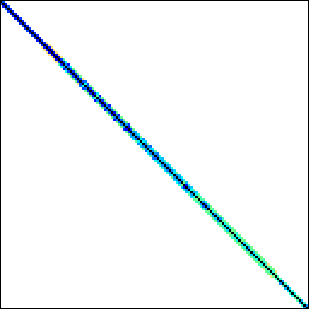
\includegraphics[width=\textwidth]{Cube_Coup_dt0}
        \caption{Cube\_Coup\_dt0}
    \end{subfigure}
    \hfill
    \begin{subfigure}[t]{0.45\textwidth}
        \centering
        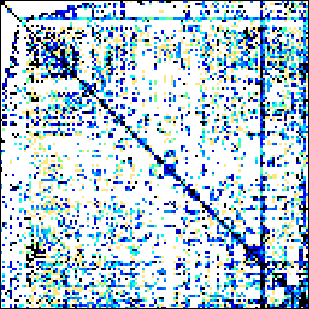
\includegraphics[width=\linewidth]{shermanACd}
        \caption{shermanACd}
    \end{subfigure}
    \caption{Well structured (a) and poorly structured (b) matrices.}
    \label{fig:Cube_Coup_dt0}
\end{figure}

\section{Shared Memory SpMV}
SpMV can be parallelized using the OpenMP directive \texttt{\#pragma omp parallel for}. By default, this tells OpenMP to use \texttt{static} scheduling when parallelizing the outer iteration loop. When static scheduling is used, the span of the iteration that each thread will execute is precomputed, and stays static, as the naming suggests. There are other scheduling options, such as \texttt{dynamic} and \texttt{guided}, which will be discussed in later sections.
\medskip

An implementation of shared memory SpMV is outlined below.
\medskip

\begin{algorithm}[H]
    \caption{Shared Memory CSR-based SpMV}
    \SetAlgoVlined
    \SetKwInOut{Input}{Input}
    \SetKwInOut{Output}{Output}
    \Input{\(A_{p},A_{j},A_{x},x\)}
    \Output{\(y\)\newline}

    \#pragma omp parallel for\\
    \For{\(i \gets 0\) \KwTo \(n\)}{
        sum \(\gets 0\)\\
        \For{\(j \gets A_{p}[i]\) \KwTo \(A_{p}[i+1]\)}{
            sum \( = \text{sum} + A_{x}[j] \cdot x[A_{j}[j]]\)\\
        }
        \(y[i] \gets\) sum
    }
    \label{alg:sharedmemoryspmv}
\end{algorithm}

\subsection{Scheduling options}
\label{sec:schedulingoptions}
As seen in \autoref{alg:sharedmemoryspmv}, the outer loop is parallelized, which translates to dividing the rows of the matrix evenly among the threads. This work fine for well structured matrices, but for matrices with dense rows, such as the matrix shown in Figure \ref{fig:staticscheduling}, we obtain large imbalances in the computational load for each thread, which impacts performance. 

\begin{figure}[H]
    \centering
    \incfig{staticscheduling}
    \caption{Row distribution among threads under static scheduling.}
    \label{fig:staticscheduling}
\end{figure}

% \subsection{Dynamic scheduling}
% With dynamic scheduling, OpenMP still precomputes the span of iterations, however threads are not assigned a specific set of iterations to execute. If thread \(A\) is assigned a set of sparse rows, and thread \(B\) is assigned a set of dense rows, then with static scheduling, \(A\) will be idle and not perform any computation while \(B\) is busy with its dense rows. With dynamic scheduling, iterations will be dynamically assigned to threads that are idle, which can distribute the workload more evenly in cases where the computational load of each iteration can differ. 
% \medskip

% At first glance, it might seem that this will fix the problem static schecduling poses in regards to workload imbalance. This can be the case on single socketed machines with few physical cores such as on a personal laptop, but as the systems that are used in this thesis are dual-socketed, and have a large number of physical cores, it is crucial to consider the impact that \textit{first touch policy} has.

% \subsection{First touch policy}
% In short, first touch policy means that the first thread to access a memory page will be the one to allocate it to its local memory. This means that if thread \(A\) accesses a memory page, and then thread \(B\) accesses the same memory page, thread \(B\) will not have access to the data in its local memory, and will have to access it from the main memory. This can lead to performance degradation if the data is accessed frequently, as accessing data from main memory is significantly slower than accessing it from local memory. 


% \subsection{Performance impact of first touch policy}
% As seen in table \ref{tab:latencynumbers}, accesses to main are significantly slower than accesses to say the L1 cache, and on dual-socketed nodes, accesses to main memory on the opposite socket have to be sent through the interlink, which is once again signicantly slower than accessing main memory. From this it becomes evident that using dynamic (or guided) scheduling is not a solution to the performance issues that might arise from poorly structured matrices.


\subsection{Dynamic Scheduling}

Dynamic scheduling in OpenMP involves precomputing the range of iterations without assigning specific iteration subsets to individual threads in advance. Under static scheduling, if thread \(A\) receives sparse rows and thread \(B\) receives dense rows, thread \(A\) will become idle prematurely while thread \(B\) remains computationally engaged. In contrast, dynamic scheduling allocates iterations at runtime to threads as they become available, thus potentially balancing the computational load more effectively, particularly when iteration workloads vary significantly.

At first glance, dynamic scheduling appears to resolve the workload imbalance inherent in static scheduling, even though it comes with more overhead. While this assumption holds true on smaller systems, such as personal laptops equipped with fewer physical cores and a single processor socket, it does not readily apply to larger, dual-socket systems utilized in this thesis. Here, the first-touch memory policy becomes particularly significant.

\subsection{First-Touch Policy}
The first-touch policy stipulates that the initial thread accessing a memory page allocates this page to its local memory domain. Consequently, if thread  first accesses a memory page, it is stored locally to thread . Subsequent accesses by thread  to this page result in non-local memory access, compelling thread  to retrieve the data from either remote or main memory. Such accesses incur performance penalties due to significantly higher latency compared to local memory access.

\subsection{Performance Implications of the First-Touch Policy}

Table \ref{tab:latencynumbers} illustrates that accesses to main memory exhibit substantially higher latency compared to local cache (e.g., L1 cache) accesses. In dual-socket configurations, accessing memory residing on the remote socket involves inter-socket communication through an interlink, further exacerbating latency. Consequently, dynamic (or guided) scheduling alone does not mitigate the performance degradation arising from poorly structured matrices, as it inadvertently exacerbates memory locality issues inherent to the first-touch policy on NUMA architectures.








% This algorithm can be parallelized using shared memory parallelization using OpenMPs \texttt{\#pragma omp parallel for} directive in the following manner:
% \medskip

% \begin{algorithm}[H]
%     \caption{Sequential CSR-based SpMV}
%     \SetAlgoVlined
%     \SetKwInOut{Input}{Input}
%     \SetKwInOut{Output}{Output}
%     \Input{\(A_{p},A_{j},A_{x},x\)}
%     \Output{\(y\)\newline}

%     \textbf{\#pragma omp parallel for}\\
%     \For{\(i \gets 0\) \KwTo \(n\)}{
%         \(y[i] \gets 0\)\\
%         \For{\(j \gets A_{p}[i]\) \KwTo \(A_{p}[i+1]\)}{
%             \(y[i] \gets y[i] + A_{x}[j] \cdot x[A_{j}[j]]\)\\
%         }
%     }
% \end{algorithm}

% \section{Computational Intensity}

\section{Distributed Memory SpMV}

In distributed memory, the workload is spread across multiple nodes. Physically, each node is its own dual-socketed system, each with its own memory. If data stored on one node is needed by another node, explicit communication has to occur between the nodes. This is typically done using the Message Passing Interface (MPI).
\medskip

For distributed memory SpMV, \autoref{alg:sharedmemoryspmv} is still utilized for computing the result vector \(y\), but the matrix is split between nodes, and each node computes a local part of \(y\). The final vector has to be assembled at the end of each iteration of SpMV. 
\medskip

On distributed memory systems, the challenges discussed in \ref{sec:schedulingoptions} are still relevant, but such systems also pose challenges in regards to the communication volume between nodes. As is evident from Table \ref{tab:latencynumbers}, communication between nodes (i.e. sending bytes over the network) is slow. As communication between nodes is slow, reducing the total communication volume per iteration of SpMV is crucial for performance.

\subsection{Load Balancing}
In order to reduce the total communication volume, it is necessary to partition the graph into several part, usually one part per node, or one part per socket. The question falls on how to most effectively partition the graph in order to reduce the communication volume. Firstly, the graph partitoner needs to ensure that the size of each partition balanced according to some criterion. Usually this criterion is described as a percentage of allowed imbalance. Secondly, it needs to minimize the amount of edges that strides across partitions, or in other words, minimize the \textit{edge cut} between partitions. The endpoints of such edges is called a \textit{separator} element. Formally, a separator \(S\) in a graph \(G\) is a set of elements such that \(G \setminus S\) is a disconnected graph.
\medskip

There are no fixed criterion of the imbalance value that leads to optimal communication reduction. It is possible to assign the entire graph to one part, leaving the other parts of the partitions empty, which effectively eliminates all communication, but this is clearly not optimal as the entire computational workload is assigned to a single process, leaving all other processes with no work. Usually an imabalence value of around 3\% is sufficient for most matrices.
\medskip


\subsection{Graph Partitioners}
There are many options when it comes to picking which graph partitioner to use, each with their own benefits and drawbacks. For the experiments performed in this thesis, the METIS graph partitioner has been used. The algorithms used in for graph partitioning in METIS are based on multilevel recursive-bisection. These kinds of algorithms optimize for communication reduction by minimizing the edge-cut, while trying to keep the size difference between partitions within the constraint given by the imbalance value.
\medskip

It is worth mentioning that the problem graph partitioners are trying to solve, mainly that of a perfect bisection, is NP-Hard. Therefore the best these tools can provide us are approximations. They are however very reliable and produce good partitions that are sufficient for our usage
\medskip


The following algorithm outlines how a graph (or matrix) is partitioned and reordered. Given a matrix \(g\) stored in the CSR Format, the number of partitions \(n_{p}\), and a partition vector \(p\) of size \(n_{p} + 1\), that is to store the size of the partition such that the size of the \(i^{th}\) ranks size is given by \(p[i+1] - p[i]\).
\medskip

\begin{algorithm}[H]
    \caption{Partitioning and reordering a matrix.}
    \SetAlgoVlined
    \SetKwInOut{Input}{Input}
    \SetKwInOut{Output}{Output}
    \Input{\(g\), \(n_{p}\), \(p\) }
    \Output{Partitioned and reordered \(g\)\newline}

    \If{\(n_{p} = 1\)}{
        p[0] \(\gets\) 0 \\
        p[1] \(\gets\) \(g.n_{r}\)\\
        \KwRet \(g\) \\
    }

    partitionVector \(\gets\) METIS\_PartGraphKway(\texttt{arguments specifying constraints for partition})\\

    newId \(\gets [0] \cdot g.n_{r}\)\\
    oldId \(\gets [0] \cdot g.n_{r}\)\\
    id \(\gets\) 0 \\
    p[0] \(\gets\) 0 \\

    \For{\(r \in \left\{ 0, \dots r \right\}\)}{
        \For{\(i \in \left\{ 0, \dots , g.n_{r} \right\}\)}{
            \If {partitionVector[\(i\)] = \(r\)}{
                oldId[\(id\)] \(\gets i\)\\
                newId[\(i\)] \(\gets\) id\\
                id \(\gets\) id + 1\\
            }
        }
        partitionVector[\(r + 1\)] \(\gets\) id\\
    }

    newRowPtr \(\gets [0] \cdot g.n_{r} + 1\)\\
    newColIdx \(\gets [0] \cdot g.n_{c}\)\\
    newValues \(\gets [0] \cdot g.n_{c}\)\\


    \For{\(i \in \{0, \dots , g.n_{r}-1\}\)}{
        d \(\gets\) g.rowPtr[oldId[i]+1] - g.rowPtr[oldId[i]]\\
        newRowPtr[i + 1] \(\gets\) newRowPtr[i] + d\\

        \For{\(j \in \{0, \dots , d - 1\}\)}{
            newColIdx[newRowPtr[i] + j] \(\gets\) g.colIdx[g.rowPtr[oldId[i]] + j]\\
            newValues[newRowPtr[i] + j] \(\gets\) g.values[g.rowPtr[oldId[i]] + j]\\
        }

        \For{\(j \in \{newRowPtr[i], \dots , newRowPtr[i+1]-1\}\)}{
            newColIdx[j] \(\gets\) newId[newColIdx[j]]\\
        }
    }

    g.rowPtr \(\gets\) newRowPtr\\
    g.colIdx \(\gets\) newColIdx\\
    g.values \(\gets\) newValues\\

    \KwRet g\\



\end{algorithm}


% In order to reduce the total communication volume, tools such as graph partiotioners or hypergraph partitioners are often used. These tools
% A big factor in reducing the communication volume 

% In a distributed memory system, it is important to partition the matrix so that the computational workload is evenly divided among the processes. This is typically achieved through the use of graph partitioning tools. A widely used tool for this purpose is METIS, which provides the function \texttt{METIS\_PartGraphKway}. Given a parameter \(nprocs\), representing the number of procsses the program will run on, \texttt{METIS\_PartGraphKway} attempts to partition the graph into \(nprocs\) equally sized parts. Since finding an optimal partition is an NP-hard problem, METIS does not guarantee an optimal solution, but it produces high-quality approximations that are sufficient for practical use.

% \subsection{Separator}
% When a graph is partitioned into different parts, there will inevitably be some edges which strides across different partitions. The endpoints of these edges are called separators, and will become important when it comes to reducing the communication load of the SpMV computation.
